\documentclass[12pt,a4paper]{article}
\usepackage{fontspec}
\setmainfont{Times New Roman}
\setsansfont{Arial}
\setmonofont{Courier New}
\usepackage[provide=*,english,romanian]{babel}
\usepackage{amsmath,amssymb,graphicx,geometry,setspace}
\usepackage{fancyhdr,caption,float,listings,xcolor,booktabs,longtable,array,calc}
\usepackage{subcaption,etoolbox,upquote}
\usepackage[unicode,hidelinks]{hyperref}
\geometry{top=2cm,bottom=2cm,left=2.5cm,right=2.5cm}
\setstretch{1.5}
\setlength{\parindent}{0pt}
\setlength{\parskip}{5pt}
\makeatletter
\renewcommand\section{\@startsection{section}{1}{0pt}{16pt}{7pt}{\normalfont\Large\bfseries}}
\renewcommand\subsection{\@startsection{subsection}{2}{0pt}{12pt}{5pt}{\normalfont\large\bfseries}}
\renewcommand\subsubsection{\@startsection{subsubsection}{3}{0pt}{9pt}{4pt}{\normalfont\normalsize\bfseries}}
\makeatother
\setcounter{secnumdepth}{-1}
\pagestyle{fancy}
\fancyhf{}
\rfoot{\thepage}
\renewcommand{\headrulewidth}{0pt}
\setlength{\headheight}{15pt}
\captionsetup{font=small,labelfont=bf,skip=6pt,justification=raggedright,singlelinecheck=false}
\captionsetup[figure]{position=above}
\lstset{language=C,basicstyle=\ttfamily\fontsize{9.5}{11.5}\selectfont,
  columns=fullflexible,showstringspaces=false,tabsize=2,numbersep=8pt,
  frame=single,rulecolor=\color{black!35},breaklines=true,keepspaces=true,
  xleftmargin=4pt,xrightmargin=4pt,aboveskip=8pt,belowskip=8pt}
\AtBeginEnvironment{lstlisting}{\singlespacing}
\AtBeginEnvironment{longtable}{\small\singlespacing}
\setlength{\emergencystretch}{3em}
\providecommand{\tightlist}{\setlength{\itemsep}{0pt}\setlength{\parskip}{0pt}}
\providecommand{\passthrough}[1]{#1}
\providecommand{\pandocbounded}[1]{#1}
\hypersetup{pdftitle={Sisteme de operare — Laborator 17},pdfauthor={Tacu Igor}}
\clubpenalty=10000
\widowpenalty=10000
\displaywidowpenalty=10000
\begin{document}
\begin{titlepage}
\thispagestyle{empty}
\begin{center}
\setstretch{1.18}

\includegraphics[width=0.23\textwidth]{scripts/report-style/utm-logo.png}\\[12pt]
\textbf{MINISTERUL EDUCAȚIEI ȘI CERCETĂRII}\\
\textbf{AL REPUBLICII MOLDOVA}\\[4pt]
\textbf{Universitatea Tehnică a Moldovei}\\
\textbf{Facultatea de Calculatoare, Informatică și Microelectronică}\\
\textbf{Departamentul Inginerie Software și Automatică}\\[36pt]
{\fontsize{22}{26}\selectfont\textbf{Raport}}\\[10pt]
Lucrare de laborator nr. 17\\[8pt]
\textbf{\large Sisteme de operare}\\[24pt]
\textbf{Tema:} Memorie partajată și condiții de cursă între fire Linux
\end{center}
\vfill
\begin{flushright}
\setstretch{1.25}
Realizat de:\\
stud. gr. FAF-242, Tacu Igor\\[24pt]
Verificat de:\\
Reițman Patricia
\end{flushright}
\vfill
\begin{center}\textbf{Chișinău – 2026 }\end{center}
\end{titlepage}

\setcounter{page}{1}
\section{Scopul lucrării}\label{scopul-lucrux103rii}

Observarea memoriei partajate între fire POSIX și a actualizărilor
pierdute la incrementarea neprotejată a unui contor.

\section{Sarcina lucrării}\label{sarcina-lucrux103rii}

\begin{itemize}
\tightlist
\item
  Compilarea și executarea repetată a variantei cu două fire.
\item
  Compararea rezultatelor cu patru fire și cuantificarea pierderilor
  observate.
\item
  Explicarea celor trei pași ai incrementării și propunerea unei
  protecții prin excludere mutuală.
\end{itemize}

\section{Considerații teoretice}\label{consideraux21bii-teoretice}

Firele aceluiași proces partajează variabilele globale, dar au stive
proprii. O incrementare obișnuită nu asigură atomicitatea secvenței
citire--modificare--scriere. Accesul concurent neprotejat constituie un
data race în C; un mutex comun poate serializa operația completă.

\section{Implementare. Rezultate
practice}\label{implementare.-rezultate-practice}

\subsection{Environment and method}\label{environment-and-method}

The supplied Lab 17 handout asks for an unprotected shared counter, a
four-thread variation, and three Observe answers. The implementation
follows that experiment. {\ttfamily\fontsize{10}{12}\selectfont fire.c}
defaults to two POSIX threads;
{\ttfamily\fontsize{10}{12}\selectfont make} also compiles the same
source as {\ttfamily\fontsize{10}{12}\selectfont fire4} with
{\ttfamily\fontsize{10}{12}\selectfont -DTHREADS=4}. Each worker
performs one million increments. Stable ID objects are passed by
address, and pthread creation/join errors are checked. The counter is
deliberately unprotected, as required.

Real runs were executed on 24 November 2026 on the Ubuntu server: x86-64
Linux 6.8.0-142-generic, glibc 2.39, GCC 13.3.0. Both variants were
built with
{\ttfamily\fontsize{10}{12}\selectfont -std=c11 -Wall -Wextra -O0 -pthread},
without compiler diagnostics. Ten executions of each variant were
recorded by
{\ttfamily\fontsize{10}{12}\selectfont run-experime\allowbreak{}nts.py}.
The raw commands and output are in
{\ttfamily\fontsize{10}{12}\selectfont evidence/exe\allowbreak{}cution.txt};
all twenty observations are in
{\ttfamily\fontsize{10}{12}\selectfont evidence/res\allowbreak{}ults.json}.

The implementation and checks were prepared with coding assistance.
These are actual automated terminal executions. Three supplied native
Terminal captures document compilation and two-thread runs, four-thread
runs, and the source/build configuration. All three are embedded below;
{\ttfamily\fontsize{10}{12}\selectfont CAPTURES.md} retains the
reproduction commands.

\subsection{Part 1 --- One shared counter, two
threads}\label{part-1-one-shared-counter-two-threads}

The experimental core is:

\par\noindent\begin{minipage}{\linewidth}

\begin{lstlisting}[language=C]
long counter = 0;
static void *work(void *arg)
{
    long id = *(long *)arg;
    printf("thread %ld sees counter = %ld\n", id, counter);
    for (int i = 0; i < N; i++)
        counter++;  /* deliberately unprotected */
    return NULL;
}
\end{lstlisting}

\end{minipage}\par

The first recorded execution produced:

\par\noindent\begin{minipage}{\linewidth}

\begin{lstlisting}
$ ./fire
thread 1 sees counter = 0
thread 2 sees counter = 4593
expected: 2000000
counter: 1258330    (lost updates: the race)
\end{lstlisting}

\end{minipage}\par

\textbf{Observe 1 --- What does the non-zero starting counter show?}
Thread 2 read 4,593 from the same global object already modified by
thread 1. Both workers belong to one process and access one shared
address space; each does not receive a private copy of the global
counter. Their automatic variables and call stacks remain separate. This
observed read illustrates sharing, but the unprotected access is a data
race and is not a valid synchronization protocol or a guarantee of
timely visibility in portable C.

\textbf{Observe 2 --- Why are updates lost and results different?}
Conceptually, {\ttfamily\fontsize{10}{12}\selectfont counter++} reads
the old value, adds one, and writes the result. If both workers read
100, compute 101, and then both write 101, two increments leave only one
visible update. Scheduling changes the overlap between these steps, so
the measured totals vary.
{\ttfamily\fontsize{10}{12}\selectfont pthread\_join} ensures that main
waits for both workers to finish; it does not make their preceding
increments mutually exclusive.

The C language gives a data race undefined behavior. Therefore, the
handout's ``always less than two million'' describes its intended
demonstration, not a universal bound. A run reaching the expected value
would not prove the program correct.
{\ttfamily\fontsize{10}{12}\selectfont -O0} helps expose the intended
read--modify--write experiment; it does not repair it, and
{\ttfamily\fontsize{10}{12}\selectfont volatile} would not repair it
either.

\subsection{Native Terminal evidence --- build and two-thread
race}\label{native-terminal-evidence-build-and-two-thread-race}

\par\medskip\noindent\begin{minipage}{\linewidth}\setstretch{1.0}
\captionof*{figure}{Figura 1. Native Terminal: working directory, compilation and three two-thread executions}
\centering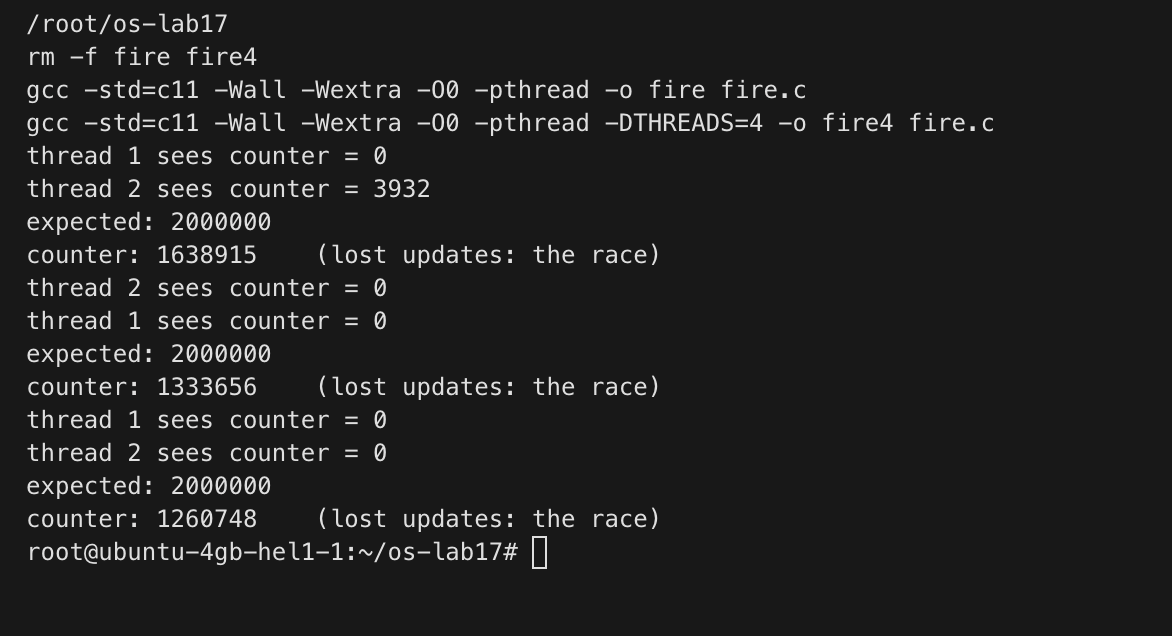
\includegraphics[width=\linewidth,height=0.67\textheight,keepaspectratio]{Lab17/evidence/screenshots/lab17-two-threads-terminal.png}
\end{minipage}\par\medskip

The supplied capture shows
{\ttfamily\fontsize{10}{12}\selectfont /root/os-lab\allowbreak{}17},
compilation of both executables with
{\ttfamily\fontsize{10}{12}\selectfont -O0 -pthread}, and three
two-thread totals: 1,638,915; 1,333,656; and 1,260,748. Relative to
2,000,000, these runs lost 361,085; 666,344; and 739,252 increments.
They are subsequent interactive observations, separate from the ten-run
series below.

In the first captured run, thread 2 initially reads 3,932 after thread 1
reads zero. In the next two runs, both initial reads are zero, yet the
final totals still lose updates. Thus the initial diagnostic may precede
the conflicting loop updates; two zero starting reads do not imply
separate memory or an absence of a race. Thread 2 prints before thread 1
in the second run, illustrating that creation order does not fix their
execution order.

\subsection{Part 2 --- Four workers and the observed
loss}\label{part-2-four-workers-and-the-observed-loss}

The additional executable changes only the worker count:

\par\noindent\begin{minipage}{\linewidth}

\begin{lstlisting}
gcc -std=c11 -Wall -Wextra -O0 -pthread -o fire fire.c
gcc -std=c11 -Wall -Wextra -O0 -pthread -DTHREADS=4 -o fire4 fire.c
\end{lstlisting}

\end{minipage}\par

Four workers should collectively perform 4,000,000 increments. The first
four-worker run ended at 2,721,928, losing 1,278,072 relative to that
target. The complete measured series is:

{\def\LTcaptype{table} % do not increment counter
\begin{longtable}[]{@{}lrrrr@{}}
\toprule\noalign{}
Run & Two threads: counter & Lost & Four threads: counter & Lost \\
\midrule\noalign{}
\endhead
\bottomrule\noalign{}
\endlastfoot
1 & 1,258,330 & 741,670 & 2,721,928 & 1,278,072 \\
2 & 1,073,256 & 926,744 & 2,220,999 & 1,779,001 \\
3 & 1,361,266 & 638,734 & 2,930,129 & 1,069,871 \\
4 & 1,440,973 & 559,027 & 2,400,952 & 1,599,048 \\
5 & 1,270,174 & 729,826 & 3,081,305 & 918,695 \\
6 & 1,277,940 & 722,060 & 2,802,551 & 1,197,449 \\
7 & 1,093,547 & 906,453 & 2,816,857 & 1,183,143 \\
8 & 1,090,006 & 909,994 & 1,559,066 & 2,440,934 \\
9 & 1,614,546 & 385,454 & 1,680,003 & 2,319,997 \\
10 & 1,626,304 & 373,696 & 1,414,598 & 2,585,402 \\
\end{longtable}
}

The two-thread mean was 1,310,634.2, corresponding to 689,365.8 missing
increments or 34.47\% of the target. The four-thread mean was
2,362,838.8, corresponding to 1,637,161.2 missing increments or 40.93\%.
Both absolute and relative mean loss increased in these ten-run samples.
The first four-thread run happened to have a lower relative loss than
some two-thread runs; the experiment does not establish monotonic loss
for every individual execution or other machines.

\subsection{Native Terminal evidence --- four-thread
race}\label{native-terminal-evidence-four-thread-race}

\par\medskip\noindent\begin{minipage}{\linewidth}\setstretch{1.0}
\captionof*{figure}{Figura 2. Native Terminal: three four-thread executions with a target of four million increments}
\centering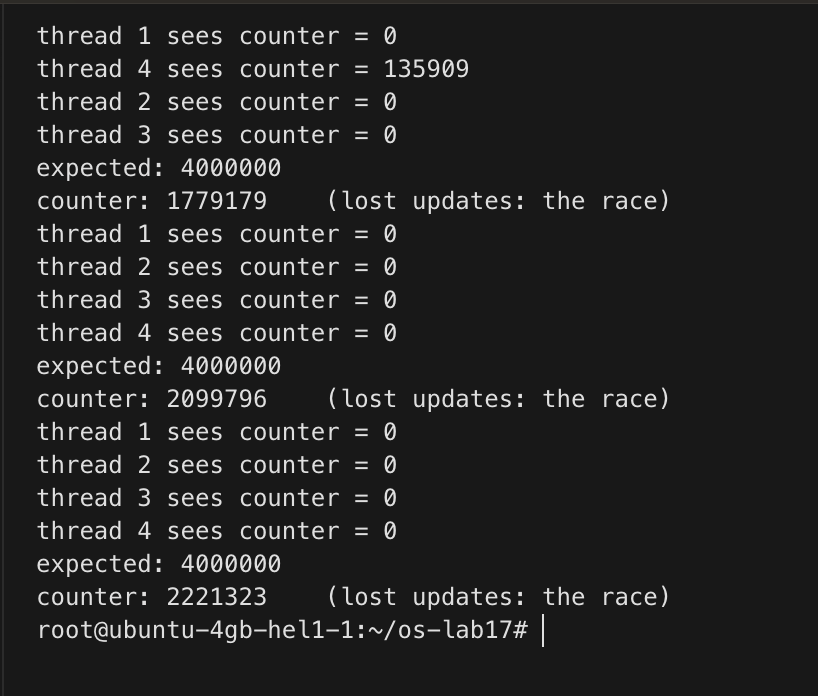
\includegraphics[width=\linewidth,height=0.67\textheight,keepaspectratio]{Lab17/evidence/screenshots/lab17-four-threads-terminal.png}
\end{minipage}\par\medskip

The three captured four-thread totals are 1,779,179; 2,099,796; and
2,221,323. They lost 2,220,821; 1,900,204; and 1,778,677 increments,
respectively, relative to 4,000,000. These are subsequent interactive
runs, separate from the ten-run sample in the table. Their mean loss is
1,966,567.3, or 49.16\% of the target; the earlier three captured
two-thread runs lost 29.44\% on average. The captured samples therefore
also show greater relative loss with four workers, without establishing
a per-run guarantee.

In the first captured run, thread 4 prints a non-zero initial value of
135,909 while other workers print zero. Their output order does not
identify the exact order of the underlying counter reads: a worker may
read an argument to printf and then wait before printing. In the
following two runs all four initial diagnostics are zero, yet both
totals remain well below the target. The conflicting accesses occur
throughout the increment loops, not only at startup.

\textbf{Observe 3 --- One-sentence fix.} Make the complete increment a
mutually exclusive critical section, for example by having every worker
lock the same mutex before
{\ttfamily\fontsize{10}{12}\selectfont counter++} and unlock it
afterwards.

A proposed implementation would surround the increment with:

\par\noindent\begin{minipage}{\linewidth}

\begin{lstlisting}[language=C]
pthread_mutex_lock(&counter_lock);
counter++;
pthread_mutex_unlock(&counter_lock);
\end{lstlisting}

\end{minipage}\par

The mutex must be initialized before starting workers and shared by all
of them. Reads during worker execution also need the same protection if
they access a counter being changed. The final read after all joins is
already sequenced after worker completion. The handout asks for the fix
as a proposal; the submitted
{\ttfamily\fontsize{10}{12}\selectfont fire} and
{\ttfamily\fontsize{10}{12}\selectfont fire4} intentionally retain the
race for observation.

\subsection{Native Terminal evidence --- source and build
configuration}\label{native-terminal-evidence-source-and-build-configuration}

\par\medskip\noindent\begin{minipage}{\linewidth}\setstretch{1.0}
\captionof*{figure}{Figura 3. Native Terminal: shared counter, unprotected increment, pthread lifecycle and both Makefile targets}
\centering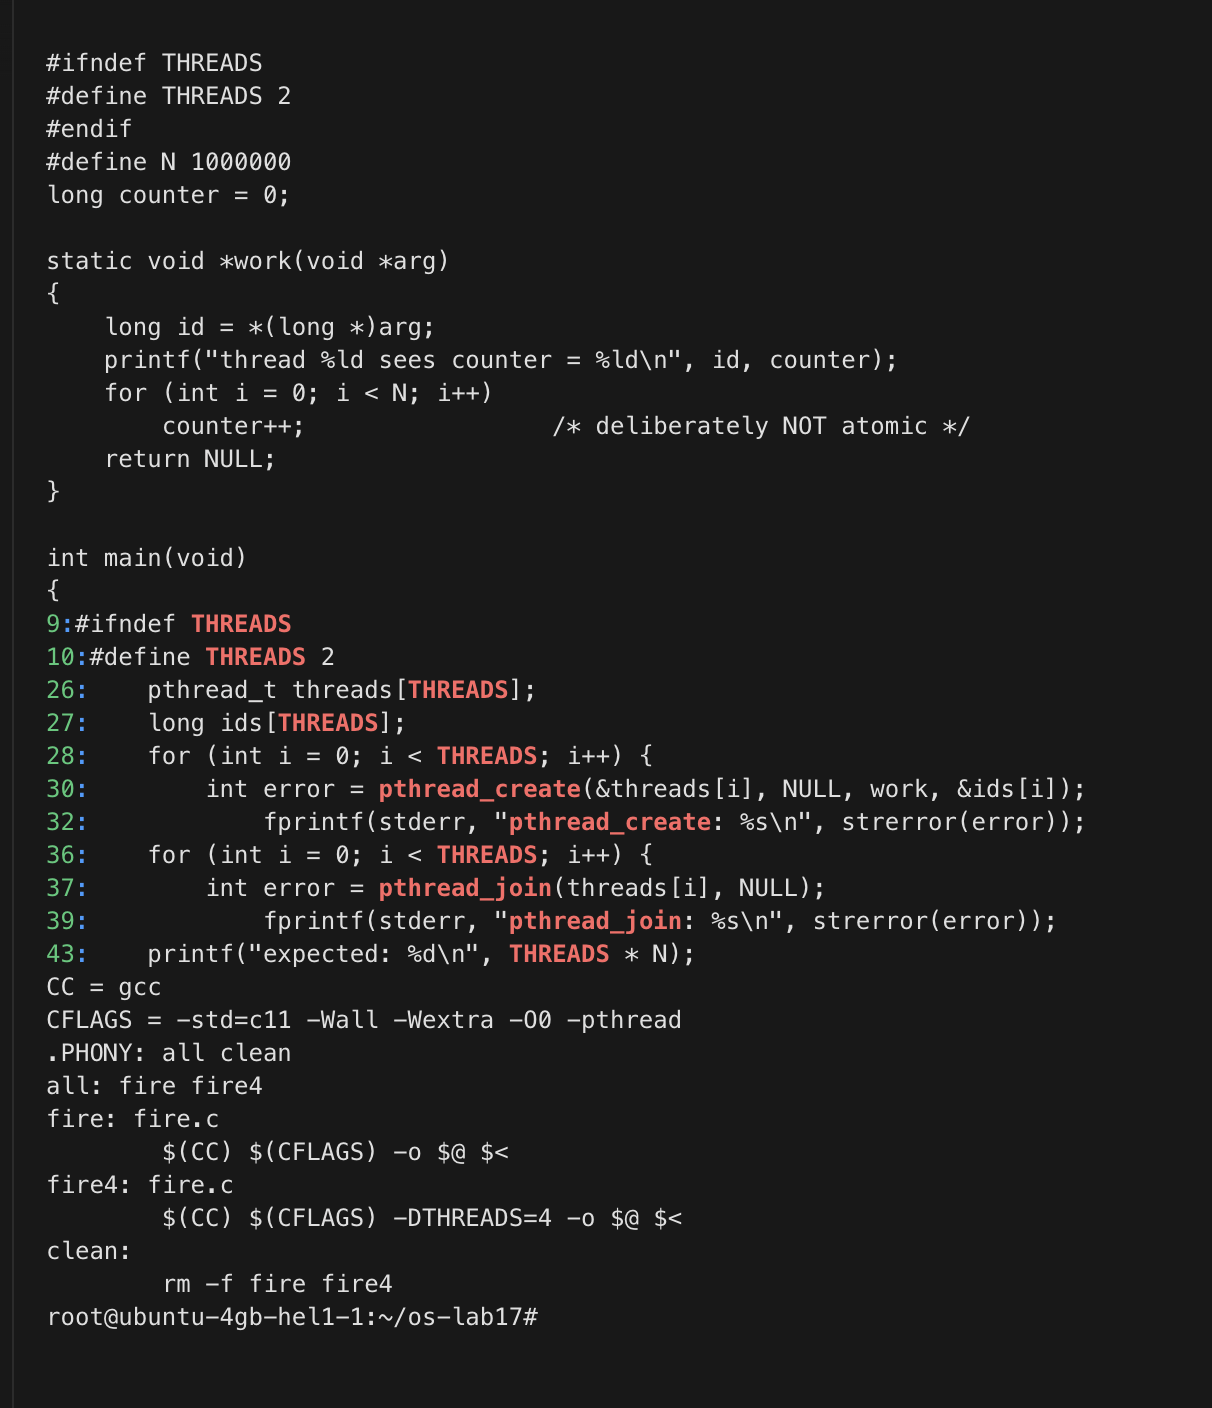
\includegraphics[width=\linewidth,height=0.67\textheight,keepaspectratio]{Lab17/evidence/screenshots/lab17-source-terminal.png}
\end{minipage}\par\medskip

The source capture shows the default
{\ttfamily\fontsize{10}{12}\selectfont THREADS=2}, one million loop
iterations per worker, the single global
{\ttfamily\fontsize{10}{12}\selectfont long counter}, and the
deliberately unprotected
{\ttfamily\fontsize{10}{12}\selectfont counter++}. It also shows one
{\ttfamily\fontsize{10}{12}\selectfont pthread\_crea\allowbreak{}te} and
one {\ttfamily\fontsize{10}{12}\selectfont pthread\_join} per worker,
with stable ID addresses passed into the worker. The Makefile compiles
the same source twice: the {\ttfamily\fontsize{10}{12}\selectfont fire4}
target overrides only the worker count with
{\ttfamily\fontsize{10}{12}\selectfont -DTHREADS=4}; both targets retain
{\ttfamily\fontsize{10}{12}\selectfont -O0 -pthread}. Thus the
comparison uses the same counter operation and loop length per worker.
The excerpt confirms the absence of a lock in the experimental loop; the
mutex snippet above is a proposed fix, not the submitted racy baseline.

\subsection{Reproduction and native
captures}\label{reproduction-and-native-captures}

On Linux, run {\ttfamily\fontsize{10}{12}\selectfont make clean all},
then {\ttfamily\fontsize{10}{12}\selectfont ./fire} and
{\ttfamily\fontsize{10}{12}\selectfont ./fire4} repeatedly. To repeat
the saved twenty-run procedure, run
{\ttfamily\fontsize{10}{12}\selectfont python3 run-experime\allowbreak{}nts.py};
it replaces the local evidence files with the newly observed values.
Follow {\ttfamily\fontsize{10}{12}\selectfont CAPTURES.md} for separate
build/two-thread, four-thread and source screenshots. Keep genuine
values even when they differ from this recorded sample.

\par\noindent\begin{minipage}{\linewidth}

\section{Concluzie}\label{concluzie}

În eșantionul măsurat, patru fire au pierdut în medie mai multe
actualizări, atât absolut, cât și procentual. Rezultatele ilustrează
partajarea și cursa, fără a garanta o anumită valoare pentru fiecare
execuție. Excluderea mutuală asupra întregii incrementări este remediul
propus.

\end{minipage}\par

\end{document}
